\section{Kinetisk energi}
Dette kan vises ved først at definere massemidtpunktets hastighed
\begin{equation} \label{eq:v_cm}
    \v{v}_\textsc{cm}=\frac{\sum m_i\v{v}_i}{\sum m_i}
\end{equation}
Det skal med henblik på udledningen bemærkes at, der om summer gælder følgende
\begin{equation}
    \sum_i^n a_ic=c\sum_i^n a_i \qquad\qquad \sum_i^n\left(a_i + b_i\right) = \sum_i^n a_i + \sum_i^n b_i
\end{equation}
hvor $c$ er en størrelse, der er konstant for alle værdier af indekset $i$. $a_i$ og $b_i$ er størrelser, der afhænger af indekset $i$. I det følgende er det underforstået, hvad der summeres over, hvorfor indexet droppes. \\

Et delelements hastighed, $\v{v}_i$, kan skrives som en sum af massemidtpunktets hastighed, $\v{v}_\textsc{cm}$, og elementets hastighed ift. massemidtpunktet, $\v{v}_i'$. Af definitionen for translatorisk kinetisk energi er det $i$'te delelementets kinetiske energi
\begin{equation}
     K_i = \frac{1}{2}m_i\v{v}_i^2 = \frac{1}{2}m_i(\v{v}_\textsc{cm}^2+\v{v}_i'^2+2\v{v}_\textsc{cm}\v{v}_i')
\end{equation}
Den totale kinetiske energi bliver summen af de enkelte deles kinetiske energi, hvor de konstante led trækkes uden for summen
\begin{equation} \label{eq:Ktot}
    K_\text{tot} = \frac{1}{2}{\v{v}_\textsc{cm}}^2\sum m_i+\frac{1}{2}\sum m_i\v{v}_i'^2+\v{v}_\textsc{cm}\sum m_i\v{v}_i'
\end{equation}
Da totalmassen af et legeme er summen af massen af de enkelte masseelementer, $M=\sum m_i$, er første led i ligning \eqref{eq:Ktot} den totale translatoriske kinetiske energi for hele legemet, $K_\text{trans}$. \\

$\v{v}_i'$ er hastigheden ift. massemidtpunktet hvorved ligning \eqref{eq:Stift-Legeme} gælder. Det medfører at
\begin{equation} \label{eq:K_rot}
     \frac{1}{2}\sum m_i\v{v}_i'^2=\frac{1}{2}\sum\left(m_ir_i^2\right)\omega^2=\frac{1}{2}I\omega^2 = K_\text{rot}
\end{equation}
Her er definitionen af inertimomentet, ligning \eqref{eq:Inertimoment}, samt det faktum, at der kigges på et stift legeme, benyttet.\\
For at ligning \eqref{eq:K} giver mening, skal det sidste led i ligning \eqref{eq:Ktot} være nul. Det vises ved først at omskrive $\v{v}_i'$ i det sidste led i ligning \eqref{eq:K_rot}
\begin{equation} \label{eq:v_i}
     \v{v}_i'=\v{v}_i-\v{v}_\textsc{cm}
\end{equation}
Multipliceres ligning \eqref{eq:v_i} med $m_i$, hvorefter der summeres, opnås
\begin{equation} \label{eq:K3}
     \sum m_i(\v{v}_i-\v{v}_\textsc{cm}) = \sum m_i\v{v}_i-\v{v}_\textsc{cm}\sum m_i = \v{v}_\textsc{cm}\sum m_i - \v{v}_\textsc{cm}\sum m_i = \v{0}
\end{equation}
hvor ligning \eqref{eq:v_cm} er benyttet. \\
Kombineres ligningerne \eqref{eq:Ktot}, \eqref{eq:K_rot} og \eqref{eq:K3} får man
\begin{equation} \label{eq:KinetiskEnergi}
     K_\text{tot} = \frac{1}{2}M{v_{\text{cm}}}^2 + \frac{1}{2}I_{\text{cm}}\omega^2 + \v{v}_{\text{cm}} \cdot \v{0} = K_{\text{trans}} + K_{\text{rot}}
\end{equation}
hvor $I_\textsc{cm}$ er inertimomentet for rotationen om en akse gennem massemidtpunktet. Da ligningerne \eqref{eq:Ktrans} og \eqref{eq:Krot} opfylder ligning \eqref{eq:K} giver definitionen af  rotationel kinetisk energi mening.

\begin{figure}[]
\centering
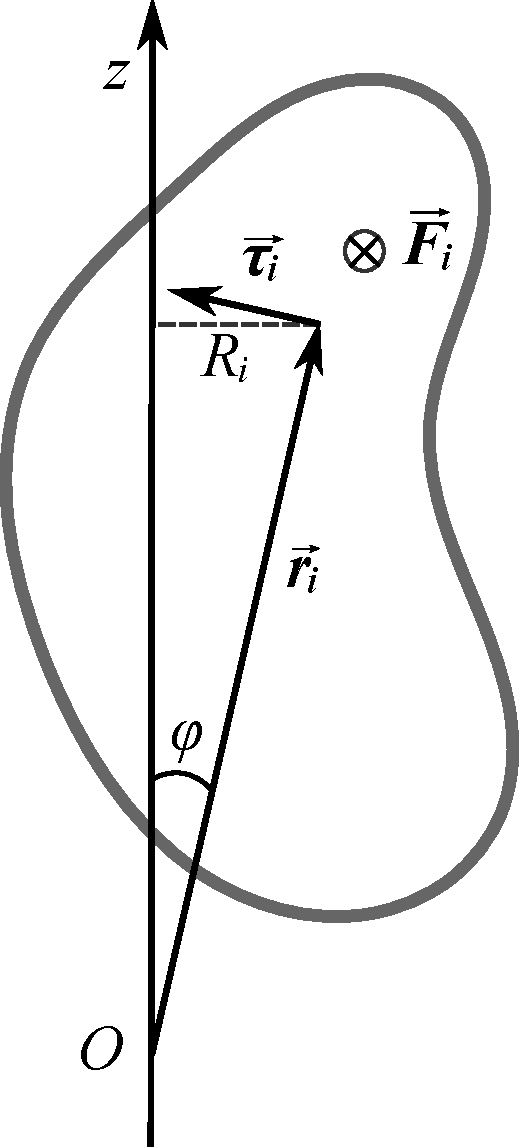
\includegraphics[width=.4\textwidth]{Analytisk-Mekanik/N2}
\caption{Arbitrært stift legeme, hvor kraften, $\v{F}_i$, peger ind i tegningen, og kraftens arm, $\v{r}_i$, er defineret ud fra punktet $O$.}
\label{fig:Kraftmoment}
\end{figure}

\subsubsection{Newtons Anden Lov for Roterende Legemer}
Newtons anden lov siger, at $\sum\v{F}=m\v{a}$, og der ønskes en tilsvarende formel for legemers resulterende kraftmoment. Der kigges nu på kraftmomentet for den $i$'te partikel i et arbitræt stift legeme, se Figur \ref{fig:Stift-legeme}. \\
Det ses, at $\v{r}_i\perp\v{F}_i$, og $\v{F}_i$ antages til at være den resulterende kraft på den $i$'te partikel, hvorfor kraftmomentets størrelse, af ligning \eqref{eq:Stift-Legeme} og ligning \eqref{eq:KraftmomentNorm}, bliver
\begin{equation}
    \tau_i = r_iF_i\ = r_im_ia_i = r_im_iR_i\alpha
\end{equation}
hvor Newtons 2. lov også er brugt. $\phi$ defineres som værende vinklen mellem rotationsaksen og kraftens arm. Det ses i figur \ref{fig:Stift-legeme} at følgende sammenhæng gælder
\begin{equation}
    R_i=r_i\sin\phi
\end{equation}
Tegnes kraftmomentet associeret med $\v{F}_i$ og deles den op i en $x$- og $z$-komposant ses det at
\begin{align}
\tau_{i,z} = \tau_i\sin\phi
\end{align}
hvorved $z$-komposanten af kraftmomentet bliver
\begin{equation}
    \tau_{i,z}=m_iR_i^2\alpha_z
\end{equation}
Summeres disse komposanter af delelementernes resulterende kraftmoment fås
\begin{equation} \label{eq:N2R}
    \sum\tau_{i,z}=\alpha_z\sum m_iR_i^2=I_z\alpha_z
\end{equation}
hvor $I_z$ er legemets inertimoment ved rotation om rotationsaksen. \\
Hvis legemet er symmetrisk omkring den givne rotationsakse bliver
\begin{equation} \label{eq:N2Rot}
    \sum\gv{\tau}_{i}\parallel \zhat \quad\Rightarrow\quad \sum\tau_{i}=I_z\alpha_z
\end{equation}
Ligning \eqref{eq:N2R} kaldes ofte for Newtons anden lov for rotationel bevægelse, og koordinatsystemet skal fastholdes under hele bevægelsen for, at ligningerne \eqref{eq:N2R} og \eqref{eq:N2Rot} gælder.